\documentclass{tufte-handout}
\usepackage{amsmath}
\usepackage[utf8]{inputenc}
\usepackage{pdfpages}
\usepackage{mathpazo}
\usepackage{booktabs}
\usepackage{microtype}

\pagestyle{empty}


\title{Flow Report}
\author{Anatoli Cooper and Boris Marley}

\begin{document}
  \maketitle

  \section{Results}

  Our implementation successfully computes a flow of 163 on the input file, confirming the analysis of the American enemy.

  We have analysed the possibilities of decreasing the capacities near Minsk.
  Our analysis is summaries in the following table:

\bigskip
  \begin{tabular}{rccc}\toprule
    Case & 4W--48 & 4W--49 & Effect on flow \\\midrule
    1& 30& 20 & no change \\
    2& 20& 30 & no change \\
    3& 20& 20 & no change \\
    4& 10& 30 & no change \\
    5& 30& 10 & no change \\
    6& 10& 10 & $-20$ \\\bottomrule
  \end{tabular}
  \bigskip

  In cases 3-6, the new bottleneck becomes
  \begin{quote}
      47--46, 48--4W, 49--4W, 49--5, 50--7, 51--7, 51--52, 51--R, H--R
  \end{quote}
  In cases 3-5, the flow is still 163, but out algorithm chooses the new cut.
  The comrade from Minsk is advised to choose case 6, since it is the only one that reduces the overall flow.

  \section{Implementation details}

  We use a straightforward implementation of Ford-Fulkerson flow algorithm as described in Bronstein, \emph{Foundations of Algorithms}, chap.~6.
  We use Depth-first-search to find an augmenting path.

  The running time is $O(v*e)$.

  We have only implemented the residual graph, which the input is parsed directly to. Each residual edge is directed and created together with a counterpart. When the flow through a edge is updated, it updates it counterpart by the difference. You can then get the original capacity by just summing its own flow and its counterpart's flow.
  Our datatype for edge is this:
  \begin{verbatim}
    class RestDiEdge
    {
      Vertex from, to;
      RestDiEdge counterpart;
      int value;
      
      void setRestValue(int);
      void setValue();
      int getCapacity();
      int getValue(); 
    }
  \end{verbatim}

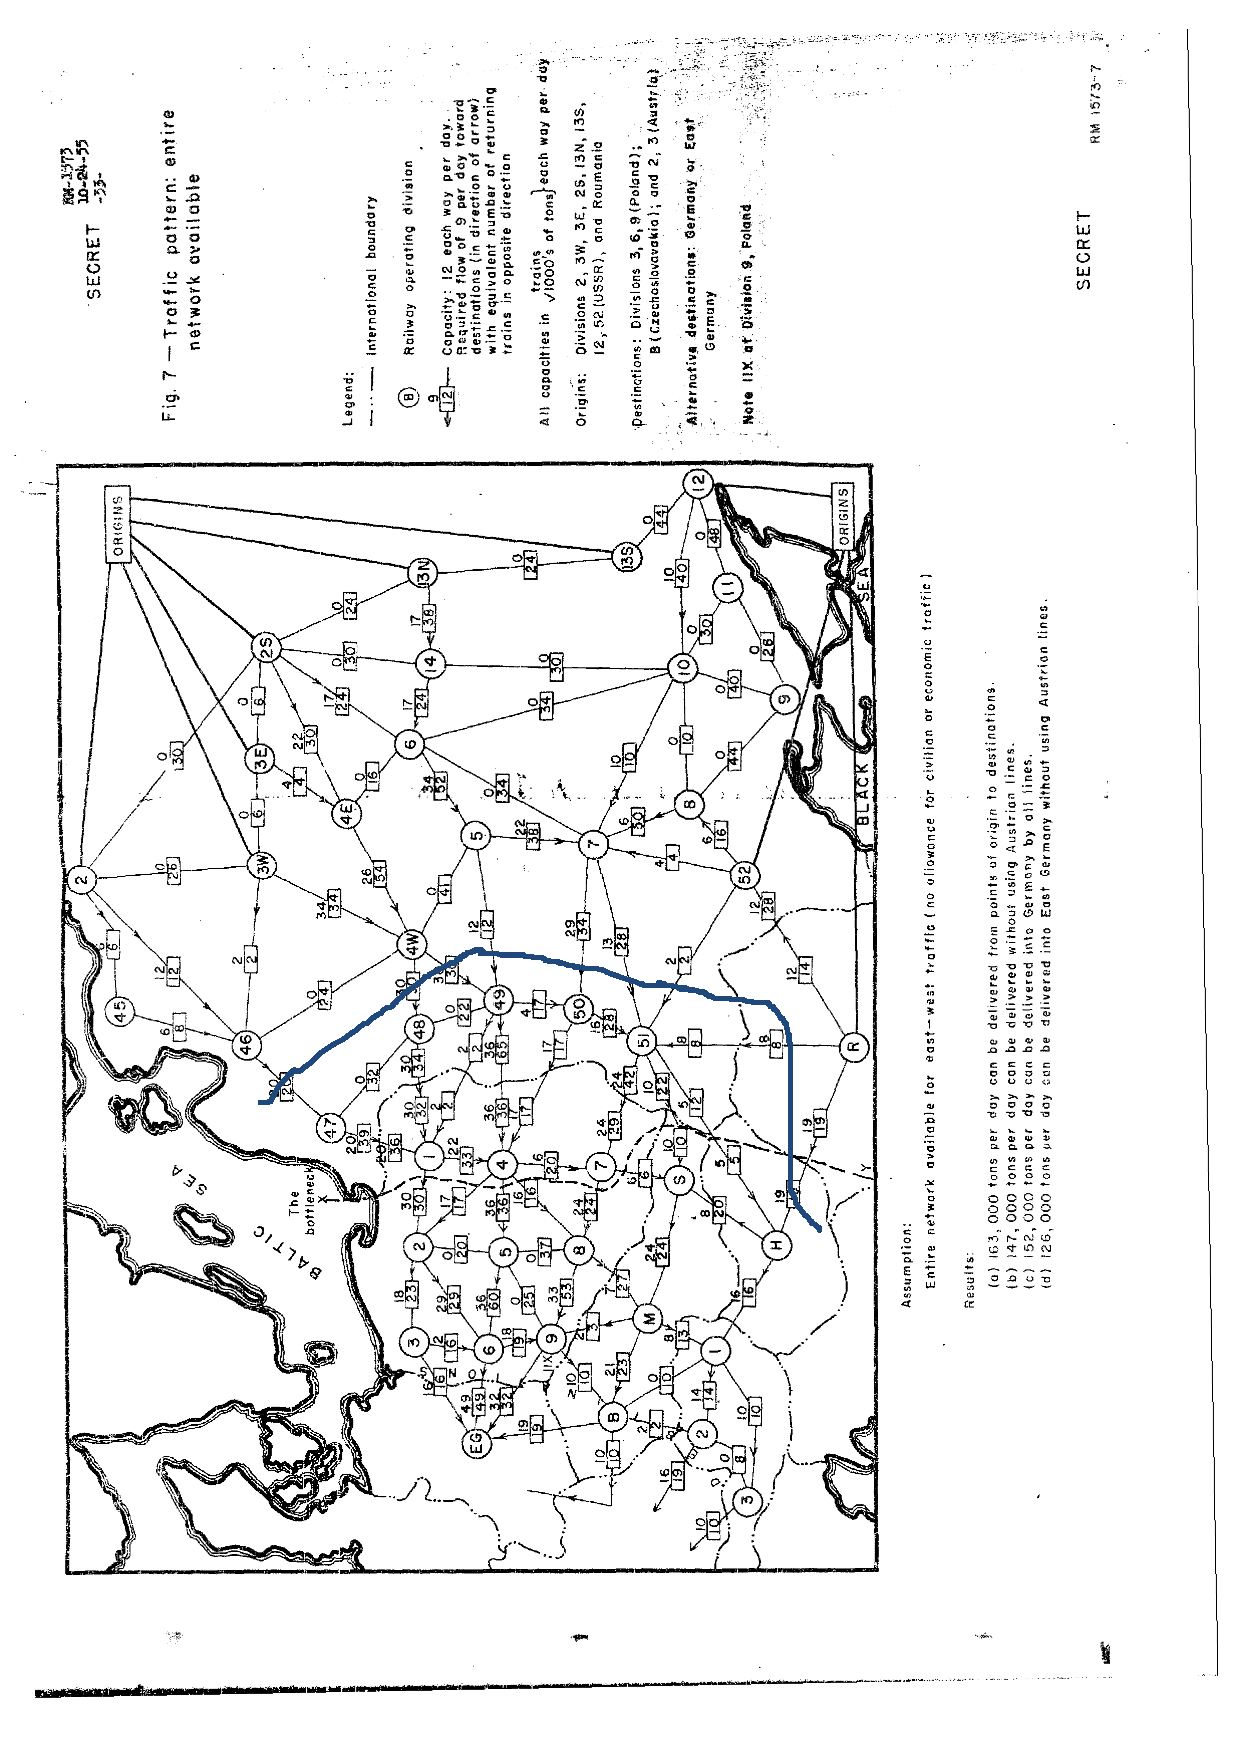
\includepdf{secret2.pdf}

\end{document}
